\chapter{Architecture Overview}

\section{Partitioning}

\begin{center}
	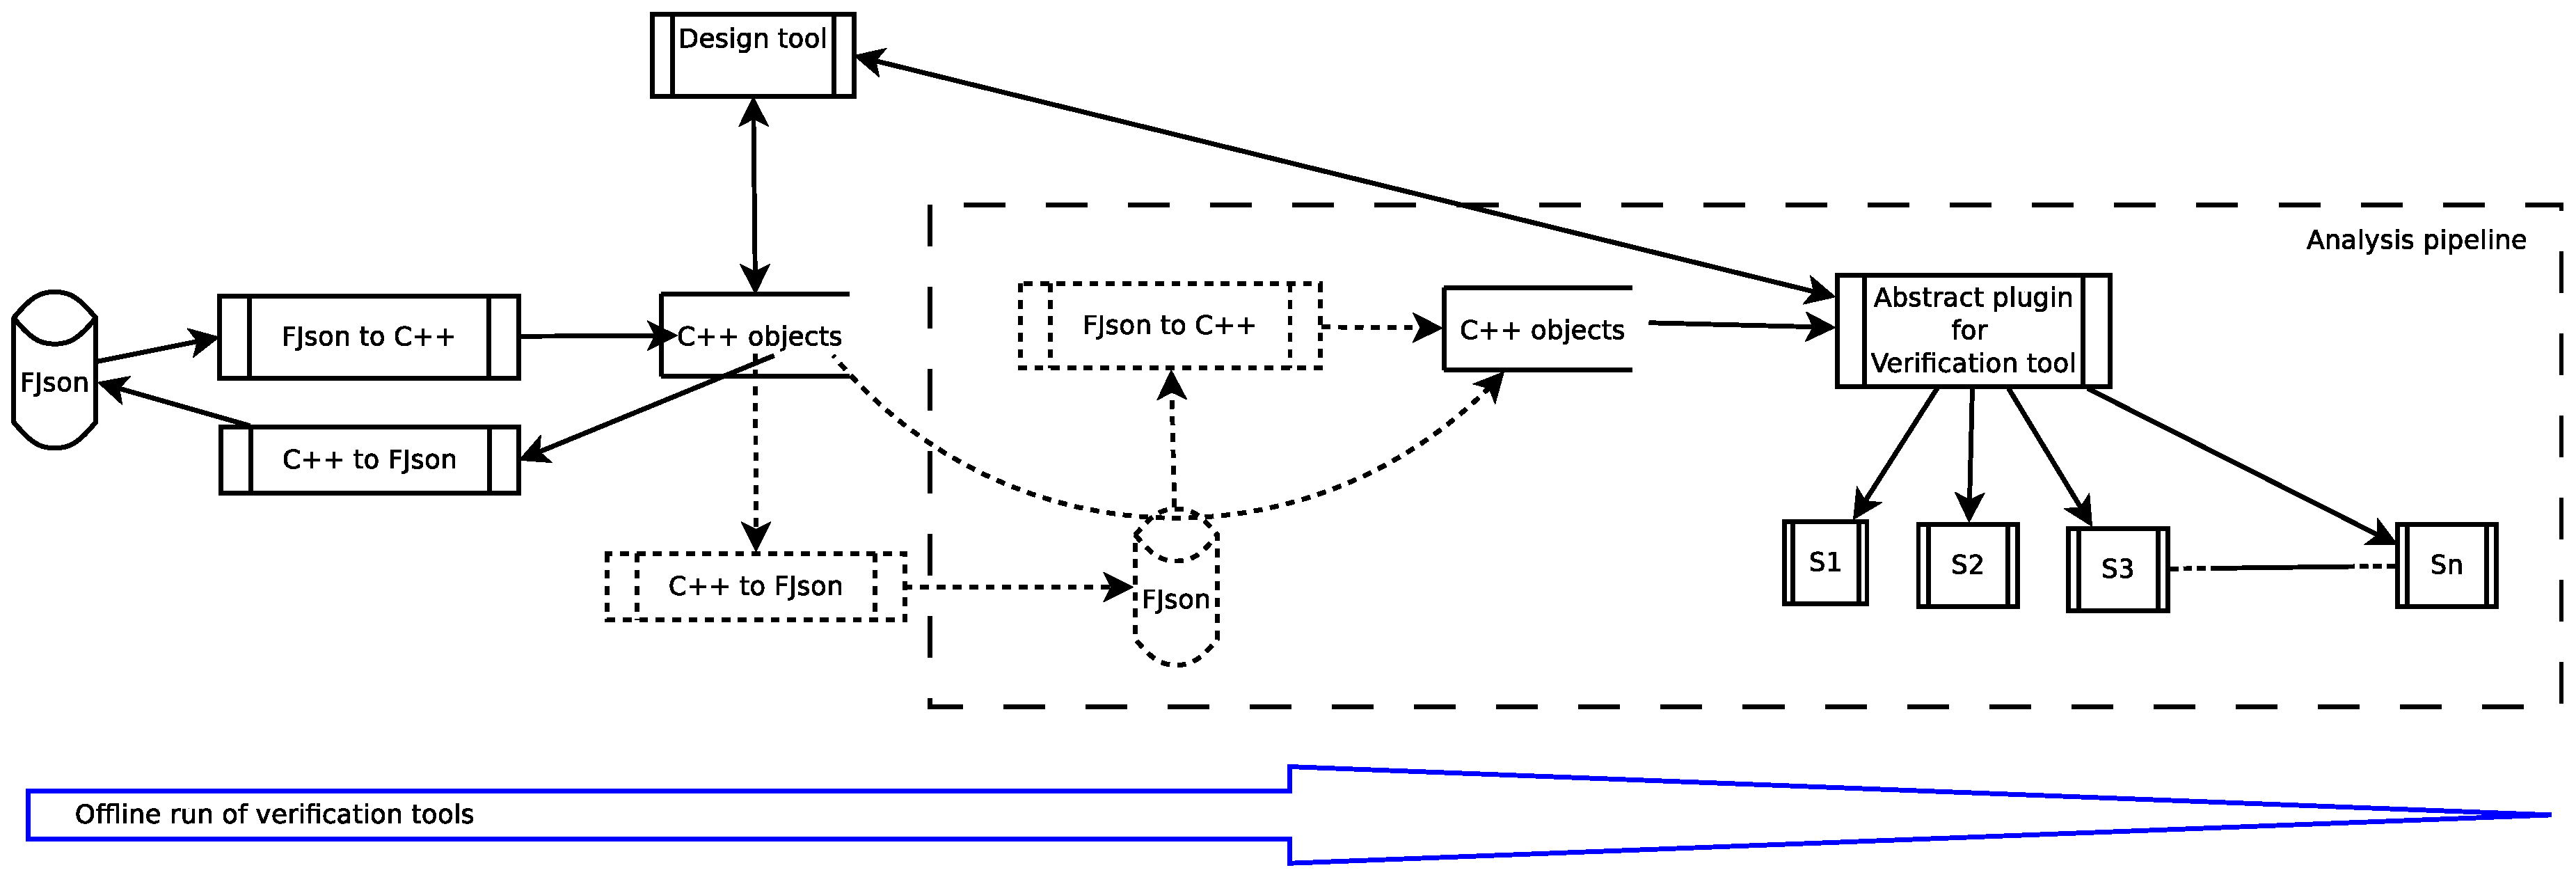
\includegraphics[width=.9\linewidth]{architecture-tool-scope}
\end{center}

The complete tool consists of a verification pipeline and
the graphical user interface where the research people
can design a Network on Chip (\Noc). Both partitions have differing
use cases. 

The use case for the verification pipeline is for verifying a model 
that needs a final check, or for verifying a model that is too 
big to verify completely during graphical edit cycles.

The use case for the graphical editor is for creating, modifying 
and intermediately verifying the \Noc. The editor allows for 
selecting verification tools to run, and will verify parameters
before each run.

The verification tools and the graphical toolkit communicatie 
through a plugin architecture.

\section{Graphical Design Tool}

The graphical editor of \Noc consists of a toolkit containing
the \xmas primitives, the composites available in separate 
libraries, and the graphical window, and the commands to 
prepare and execute the verification tools.

The process of designing an \Noc consists of alternating edit-verify cycles.
Once the model is finished, all parameters per component are filled in, the 
verify tools are selected, the the controller will copy the current model and
kick off the verification tools for an execution run.

\begin{center}
	\includegraphics[width=.9\linewidth]{../architecture-dynamic}
	\captionof{figure}{Dynamic process of editing and verifying}
	\label{fig:dynamic-arch}
\end{center}

\section{Verification pipeline}

For the graphical editor the verification pipeline itself is
not in scope. The connection to the verification pipeline is through
the plugin architecture, where a plugin is wrapped in a C++ class
that derives from \w{VerificationTool}.

Each verification tool must register with the \w{VTController} or 
the controller. The registration involves informing the
\w{VTController} about function, and parameters of the 
verification tool at hand. The graphical editor will ask the 
\w{VTController} for available verification tools.


\section{Layer architecture}

\section{Plugin communication}

\section{Primitive toolkit communication}

\section{Toolkit repository}

\section{Model repository}
